\documentclass[a4paper, 11pt]{book}
% \usepackage{/home/nora/Documents/Enseignement/Prepa/bpep/fichiers_utiles/preambule}
\usepackage{cours-preambule}

\makeatletter
\renewcommand{\@chapapp}{Kh\^olles MPSI -- semaine}
\makeatother
\renewcommand\thechapter{23}

% \toggletrue{student}
% \toggletrue{corrige}

\newcommand{\evt}{\phantom{\frac{\frac{\frac{1}{1}}{1}}{\frac{\frac{1}{1}}{1}}}}


\begin{document}

\settype{enon}
\settype{solu}

\chapter{Sujet 1\siCorrige{\!\!-- corrig\'e}}
\resetQ
\subimport{/home/nora/Documents/Enseignement/Prepa/bpep/exercices/TD/reaction_2_couples/}{sujet.tex}

\chapter{Sujet 2\siCorrige{\!\!-- corrig\'e}}
\resetQ
\subimport{/home/nora/Documents/Enseignement/Prepa/bpep/exercices/Colle/Dephosphatation_des_eaux/}{sujet.tex}

\chapter{Sujet 3\siCorrige{\!\!-- corrigé}}
\resetQ
\subimport{/home/nora/Documents/Enseignement/Prepa/bpep/exercices/TD/diagramme_pS/}{sujet.tex}

\chapter{Sujet 4\siCorrige{\!\!-- corrigé}}
\resetQ
\subimport{/home/nora/Documents/Enseignement/Prepa/bpep/exercices/TD/precipitation_ZnS/}{sujet.tex}

\chapter{Sujet 5\siCorrige{\!\!-- corrigé}}
\resetQ
% \subimport{/home/nora/Documents/Enseignement/Prepa/bpep/exercices/DS/oxyde_azote/}{sujet.tex}
\section{Pile à combustible à oxyde solide \hfill \small écrit PT 2015}
\enonce{%
Le principe de la pile à combustible consiste à utiliser du dihydrogène pour
stocker et transporter de l'énergie. Une pile à combustible est un assemblage
de cellules élémentaires, en nombre suffisant pour assurer la production
électrochimique d'électricité dans les conditions de tension et d'intensité
voulues. De façon générale, le fonctionnement électrochimique d'une cellule
élémentaire de pile à combustible peut être représenté selon le schéma de la
Figure~\ref{fig:pile_comb}
\begin{center}
	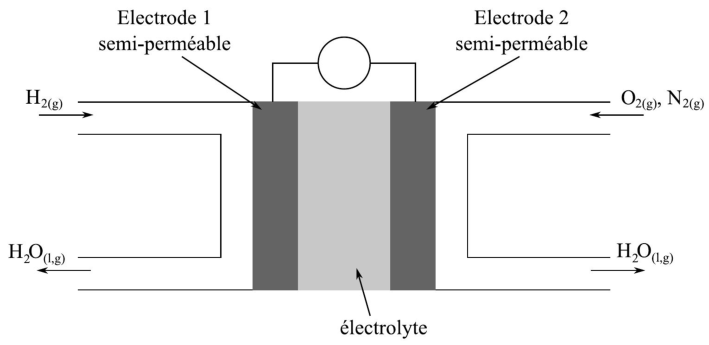
\includegraphics[width=.8\linewidth]{../figures/pile_comb}
	\captionof{figure}{Schéma de principe d'une pile à combustible.}
	\label{fig:pile_comb}
\end{center}
Chaque cellule élémentaire est constituée de deux compartiments disjoints,
alimentés chacun en gaz dihydrogène et dioxygène. Les électrodes sont séparées
par un électrolyte solide qui laisse passer les anions oxygène. Les couples
d'oxydoréduction mis en jeu dans la réaction sont
$\ce{{H}^+_{\rm(aq)}/{H_2}_{\rm(g)}}$ et $\ce{{O_2}_{\rm(g)}/H_2O_{\rm(l)}}$.
}%
\QR{%
	Indiquer la position des atomes constitutifs des réactifs et du produit dans
	le tableau périodique. En déduire leur nombre d'électrons de valence et
	ainsi les schémas de \textsc{Lewis} des trois molécules.
}{%
	L'hydrogène est dans la première ligne, première colonne donc 1 électron de
	valence et respecte la règle du duet~; l'oxygène deuxième
	ligne, 16\ieme{} colonne donc 6 électrons de valence et respecte la règle de
	l'octet. Ainsi,
	\[
		\cfig{H-H}
		\qet
		\cfig{\charge{120=\|,-120=\|}{O}=\charge{60=\|,-60=\|}{O}}
		\qet
		\cfig{\charge{45=\|,135=\|}{O}
			(-[7,.7]H)
			(-[5,.7]H)
		}
	\]
}%
\QR{%
	À partir des informations du schéma, attribuer et justifier le choix de la
	cathode et de l'anode aux électrodes 1 et 2, ainsi que le sens de circulation
	des électrons.
}{%
	Au niveau de l'électrode 1, il y a arrivée de dihydrogène, un réducteur, et
	départ d'eau, l'oxydant associé~: il y a donc \textbf{oxydation du
		dihydrogène}, et \textbf{l'électrode 1 est l'anode}. Réciproquement à
	l'électrode 2 il y a arrivée de dioxygène, un oxydant, et départ d'eau qui est
	le réducteur associé~: il y a donc \textbf{réduction du dioxygène}, et
	\textbf{l'électrode 2 est la cathode}. Ainsi, les électrons traversent la pile
	de l'électrode 1 vers l'électrode 2.
}%
\QR{%
Écrire les demi-équations électroniques pour chaque couple mis en jeu, quand
la pile débite.
}{%
D'après la question précédente,
\[
	\ce{{H_2}_{\rm(g)} -> 2 {H}^+_{\rm(aq)} + 2e^-}
	\qet
	\ce{{O_2}_{\rm(g)} + 4 {H}^+_{\rm(aq)} + 4e^- -> 2 {H_2O}_{\rm(l)}}
\]
\begin{tcb}(rema)<lftt>{Signe des demi-équations}
	Il n'est jamais faux d'écrire les demi-équations avec des signes «~=~», mais
	comme la pile débite on suppose qu'on s'intéresse au sens de
	fonctionnement~; on peut insister sur la transformation avec une flèche.
\end{tcb}
}%
\QR{%
	Le réactif qui est oxydé est appelé le combustible de la pile. Parmi les
	espèces chimiques présentes dans les couples, laquelle constitue le
	combustible~?
}{%
	Parmi les espèces en présence, c'est \textbf{le dihydrogène} qui est oxydé,
	c'est donc lui le combustible.
}%
\QR{%
En déduire l'équation de la réaction modélisant la transformation ayant lieu
dans la cellule de réaction.
}{%
En combinant les demi-équations~:
\[
	\boxed{
	\ce{
	2 {H_2}_{\rm(g)} + {O_2}_{\rm(g)} -> 2 {H_2O}_{\rm(l)}
	}
	}
\]
}%
\enonce{%
	Dans un véhicule motorisé fonctionnant grâce à une pile à combustible, on
	estime à \SI{1.5}{kg} la masse de dihydrogène nécessaire pour parcourir
	\SI{250}{km}.
}%

\QR{%
	Calculer la quantité de matière de dihydrogène correspondant à cette masse,
	puis le volume occupé par cette quantité de gaz à $\SI{20}{\degreeCelsius}$
	sous pression atmosphérique.
}{%
	La masse molaire du dihydrogène est $M_{\ce{H_2}} = \SI{2.0}{g.mol^{-1}}$~; la
	quantité de matière nécessaire pour parcourir \SI{250}{km} est donc
	\begin{gather*}
		n = \frac{m}{M} = \SI{750}{mol}
		\\\beforetext{Or, gaz parfait donc}
		\boxed{V = \frac{nRT}{P}}
		\Lra
		\xul{V = \SI{1.8e4}{L}}
	\end{gather*}
}%
\QR{%
	Quel est l'avantage pour l'environnement de l'utilisation d'une pile à
	combustible au dihydrogène par rapport à un carburant classique~? Quel en est
	l'inconvénient majeur~?
}{%
	Le gros avantage de la pile à combustible est qu'elle ne rejette que de l'eau,
	et aucune substance polluante. L'inconvénient majeur de la pile envisagée ici
	est bien sûr la production et le stockage du dihydrogène, qui est un gaz très
	explosif.
	\begin{tcb}(rema)<lftt>{Remarque}
		Le stockage du dihydrogène pour les piles à combustible est un domaine de
		recherche très actif. Il est a priori produit par électrolyse de l'eau
		(i.e.\ l'inverse de la réaction ayant lieu dans la pile), l'énergie
		nécessaire à l'électrolyse pouvant venir d'une source d'énergie propre. Il
		est ensuite stocké selon différentes modalités~: bouteille de gaz ou de
		liquide, stockage dans des hydrures métalliques solides, etc. Voir la page
		Wikipédia «~Pile à combustible~» pour plus d'informations.
	\end{tcb}
}%

\chapter{Sujet 6\siCorrige{\!\!-- corrigé}}
\resetQ
\enonce{%
	On étudie ici l'accumulateur lithium-oxyde de manganèse, qui représente
	environ 80\% du marché des batteries au lithium. La première électrode est en
	dioxyde de manganèse \ce{MnO2}, la deuxième en lithium \ce{Li}. Ces deux
	électrodes baignent dans un électrolyte organique contenant des ions \ce{Li+}.
	\begin{tcb}(data)<lfnt>{Données}
		\begin{itemize}
			\item Numéro atomique du lithium~: $Z = 3$.
			\item Masse molaire du lithium~: $M_{\ce{Li}} = \SI{5.9}{g.mol^{-1}}$.
			\item Potentiels standard~: $E_1^\circ(\ce{Li^+/Li_{\rm(s)}}) =
				      -\SI{3.03}{V}$ et
			      $E_2^\circ(\ce{{MnO_2}_{\rm(s)}/{LiMnO_2}_{\rm(s)}})$ = \SI{0.65}{V}.
		\end{itemize}
	\end{tcb}
}%
\QR{%
	Indiquer la position du lithium dans le tableau périodique. Pourquoi choisir
	un électrolyte organique plutôt que de l'eau~?
}{%
	Le lithium est situé deuxième ligne, première colonne, sous l'hydrogène. C'est
	le premier métal alcalin. Comme tous les alcalins, c'est un \textbf{très fort
		réducteur}, qui réagit violemment avec l'eau (de manière explosive).
}%
\QR{%
	Écrire les réactions aux électrodes lorsque l'accumulateur fonctionne en
	générateur, ainsi que la réaction globale de fonctionnement.
}{%
	\noindent
	\begin{minipage}[t]{.55\linewidth}
		En fonctionnement générateur, la réaction chimique a lieu dans le sens
		spontané, donc entre espèces de domaines disjoints. On trace le diagramme de
		prédominance~:
	\end{minipage}
	\hfill
	\begin{minipage}[t]{.45\linewidth}
		\vspace{0pt}
		\begin{center}
			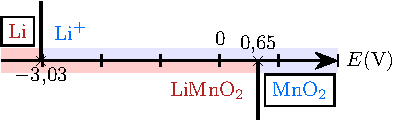
\includegraphics[width=.7\linewidth]{../figures/predom_limno}
		\end{center}
	\end{minipage}
	\smallbreak
	D'où les demi-équations~:
	\begin{align*}
		\beforetext{Électrode de lithium}
		\ce{Li_{\rm(s)}                                   & -> {Li}^+_{\rm(aq)} + e^-}
		\\\beforetext{Électrode de manganèse}
		\ce{{MnO_2}_{\rm(s)} + {Li}^+_{\rm(aq)} + e^-     & -> {LiMnO_2}_{\rm(s)}}
		\\\beforetext{Fonctionnement global}
		\ce{
		{MnO_2}_{\rm(s)} + {Li}^+_{\rm(aq)} + Li_{\rm(s)} & ->
		{LiMnO_2}_{\rm(s)} + {Li}^+
		}
		\\\beforetext{Soit}
		\ce{
		{MnO_2}_{\rm(s)} + Li_{\rm(s)}                    & ->
		{LiMnO_2}_{\rm(s)}
		}
	\end{align*}
	\begin{tcb}(rema)<lftt>{Remarque}
		L'ion lithium joue un rôle analogue à celui des ions $\ce{H^+}$ en solution
		aqueuse.
	\end{tcb}
}%
\QR{%
	La pile contient-elle un pont salin ou équivalent~? Pourquoi~?
}{%
	Les deux espèces qui réagissent sont deux solides, physiquement séparés en
	deux électrodes. Le rôle du pont salin étant d'empêcher les réactifs d'être en
	contact direct pour force le transfert d'électrons par l'extérieur du système
	(et donc être exploitables), il n'y a pas de pont salin nécessaire ici.
}%
\QR{%
	Déterminer la force électromotrice de la pile.
}{%
	\leavevmode\vspace*{-15pt}\relax
	\begin{gather*}
		E_{\ce{Li}} = E_1^\circ + \num{0.06}\log \frac{[\ce{Li^+}]}{c^\circ}
		\qet
		E_{\ce{MnO_2}} = E_2^\circ + \num{0.06} \log \frac{[\ce{Li^+}]}{c^\circ}
		\\\Ra
		e = E_{\ce{MnO_2}} - E_{\ce{Li}}
		\Lra
		\boxed{e = E_2^\circ - E_1^\circ}
		\Ra
		\xul{e = \SI{3.68}{V}}
	\end{gather*}
}%
\QR{%
	Déterminer la capacité $C$ de la pile en \si{A.h} pour une masse initiale de
	\SI{2}{g} de lithium.
}{%
	À partir de l'équation à l'électrode de lithium, on constate que lorsque la
	réaction (totale) est terminée, la quantité de matière $n$ d'électrons ayant
	transité dans le circuit est égale à la quantité de matière de lithium
	initialement introduite. D'où la charge totale~:
	\[
		\boxed{C = \frac{m_{\ce{Li}}}{M_{\ce{Li}}} \Nc_A e}
		\Ra
		\xul{C = \SI{3.2e4}{C} = \SI{9.0}{A.h}}
	\]
}%




\end{document}
